\documentclass{report}

\usepackage[sort&compress,numbers]{natbib}
\usepackage{multicol}
\usepackage{etoolbox}
\usepackage{subfig}
\usepackage{tikz}
\usetikzlibrary{
    calligraphy,
    colorbrewer,
    decorations.markings,
    decorations.pathreplacing,
    patterns,
    spy,
    }
\usepackage{float}
\usepackage[framemethod=default]{mdframed}
\usepackage[a4paper, margin=1in]{geometry}
\usepackage{enumitem}
\usepackage{xcolor}
\usepackage{graphicx}

% pgf plots and tables
\usepackage{filecontents}
\usepackage{colortbl}
\usepackage{hhline}
\usepackage{pgfplots}
\usepackage{pgfplotstable}
\pgfplotsset{compat=1.18}

% Minted for text
\usepackage{minted}
    \setminted[haskell]{
        frame=lines,
        framesep=2mm,
        linenos
    }
    \setminted[cuda]{
        frame=lines,
        framesep=2mm,
        linenos
    }

% Math symbols
\usepackage{amsmath}
\usepackage{amssymb}

\setlist{noitemsep, topsep=0pt}

\newcommand{\TODO}[1]{\noindent{\color{red}\textbf{[TODO] #1}}}
\newcommand{\floor}[1]{\left\lfloor #1 \right\rfloor}
\newcommand{\ceil}[1]{\left\lceil #1 \right\rceil}
\newrobustcmd*{\fsquare}[1]{\tikz{\filldraw[draw=#1,fill=#1] (0,0) rectangle (0.22cm,0.22cm);}}

\pgfplotstableset{
  /color cells/min/.initial=0,
  /color cells/max/.initial=1000,
  /color cells/textcolor/.initial=,
  color cells/.style={
    postproc cell content/.append code={%
          \pgfkeys{/color cells/.cd,#1}%
      \pgfkeysgetvalue{/pgfplots/table/@preprocessed cell content}\value%
      \ifx\value\empty%
      \else%
        \pgfmathfloatparsenumber{\value}\pgfmathfloattofixed{\pgfmathresult}%
        \let\value=\pgfmathresult%
        \pgfplotscolormapaccess%
            [\pgfkeysvalueof{/color cells/min}:\pgfkeysvalueof{/color cells/max}]%
            {\value}{\pgfkeysvalueof{/pgfplots/colormap name}}%
        \pgfkeysgetvalue{/pgfplots/table/@cell content}\typesetvalue%
        \pgfkeysgetvalue{/color cells/textcolor}\textcolorvalue%
        \toks0=\expandafter{\typesetvalue}%
        \edef\temp{\noexpand\pgfkeyssetvalue{/pgfplots/table/@cell content}{%
            \noexpand\cellcolor[rgb]{\pgfmathresult}%
            \noexpand\definecolor{mapped color}{rgb}{\pgfmathresult}%
            \ifx\textcolorvalue\empty\else\noexpand\color{\textcolorvalue}\fi%
            \the\toks0%
          }%
        }%
        \temp%
      \fi%
      }%
  }%
}%

\pgfplotsset{
    % this *defines* a custom colormap ...
    colormap={viridis-light}{
        rgb255=(33,145,140),
        rgb255=(34,168,132),
        rgb255=(68,191,112),
        rgb255=(122,209,81),
        rgb255=(189,223,38),
        rgb255=(254,231,36),
        rgb255=(255,255,255),
    }
}

\tikzset{
    thread/.pic={
        \draw[->,decorate, decoration={snake}] (0, 0.9) -- +(0, -0.8);
    }
}

\tikzset{
    threadblock/.pic={
        \draw (0, 0) rectangle +(2, 1);
        \foreach \x in {1,2,3,8,9,10} {
            \pic at ({\x / 5.5}, 0) {thread};
        }
        \node at (1, 0.5) [scale=0.75] {\dots};
    }
}

\tikzset{
    warp/.pic={
        \draw (0, 0) rectangle +(1, 1);
        \pic at (0.2, 0) {thread};
        \node at (0.6, 0.5) {$\times 32$};
    }
}

\tikzset{
    ->-/.style={decoration={
        markings,
        mark=at position .5 with {\arrow{>}}},postaction={decorate}
    }
}

\tikzset{
    sm_warp/.pic={
        \draw (0,  0  ) rectangle +(2, -1.0) node[pos=.5,align=center] {Warp\\Scheduler};
        \draw (0, -1  ) rectangle +(2, -0.5) node[pos=.5] {$16\times$FP32};
        \draw (0, -1.5) rectangle +(2, -0.5) node[pos=.5] { $8\times$FP64};
        \draw (0, -2  ) rectangle +(2, -0.5) node[pos=.5] {$16\times$INT32};
    }
}

\title{Improving Performance in Structured GPGPU Workloads via Specialized Thread Schedules}
\author{Naraenda Prasetya}
\date{2022}

\begin{document}

\maketitle

\chapter*{Abstract}
\TODO{Write thisss}

\tableofcontents

\chapter{Introduction}
Graphics Processing Units (GPUs) are specialized hardware that can manipulate large amounts of data in a highly parallel manner.
The hardware's main purpose is processing graphical data, however modern use of GPUs is in the form of general-pupose computing on the GPU (GPGPU) where we exploit the GPUs many cores to run computations normally run on CPUs in parallel.

This high performance GPU computing has become very accessible via high-level programming languages and libraries, which provide a limited set of operators, such as stencil, permute, fold, scan, which can manipulate data on a GPU \cite{chakravarty2011accelerating}.
An obvious drawback of high-level languages is that low-level interfaces of the hardware becomes less available as the compiler and libraries handle these.
In most cases, the compiled assembly has inefficient memory accesses with lower cache hit rates and uncoalesced accesses compared to manually tweaked code which requires in-depth knowledge about the architecture.
On the other hand, any optimization done to the compiler or library will benefit the program.
An approach that fits between improving the compiler and programmer skill, is to improve the thread scheduler.
A smarter scheduler can achieve better cache and memory utilization \cite{nugteren2014study}.
We propose a simple schedule to improve performance by leveraging the structure of memory accesses in the high level GPGPU framework Accelerate \cite{chakravarty2011accelerating}.

\section{Motivation}

\section{Contributions}
This thesis shows that the cache efficiency for stencil and matrix multiplication can be improved compared to the naive implementation and the more common tiling approach, by rescheduling via index mapping.
While the main focus lies in improving the performance on GPU, the techniques presented can also be applied on a CPU.

\vspace{1em}
The main contributions of this thesis are:
\begin{itemize}
    \item An analysis of the theoretical cache utilization and efficiency of both linear and multithreaded (GPU) execution for naive and tiled implementations of stencil and matrix multiplication operations.
    \item A simple implementeable schedule and benchmark for stencil and matrix multiplication operations that improve cache efficiency and therefore performance compared to the naive and tiling implementation.
    \item An analysis of the theoretical cache utilization and efficiency of a column-based scheduler.
\end{itemize}

\section{Outline}
We will first introduce the architecture of GPUs in chapter \ref{chap:background}: the organization of hardware, the memory hierarchy, the execution model, and the performance of certain access patterns.
A few existing optimization techniques are analysed for both stencils and matrix multiplications in chapter \ref{chap:analysis}.
We present our alternative approach and its analysis to the aforementioned optimizations in chapter \ref{chap:cbi}.
The benchmarks and results from our method are presented in chapter \ref{chap:results}.

\section{Common variable names}
\begin{itemize}
    \item $L$ Cache line size (elements)
    \item $M$ Cache size (elements)
    \item $M_L$ Cache size (number of cache lines)
    \item $F$ Memory fetches
    \item $I_w$, $I_h$ input size (number of tasks to produce the output)
    \item $S_w$, $S_w$ stencil size
\end{itemize}

\chapter{Background}
\section{GPU Architecture}
The GPU backend of Accelerate only works with CUDA capable devices (see section \ref{sec:accelerate}).
Therefore, we will mostly focus on the architecture of newer Nvidia GPUs.

\subsection{Hardware}
On modern Nvidia GPU architectures is composed of multiple GPU Processing Clusters (GPCs), Texture Processing Clusters (TPCs), Streaming Multiprocessors (SMs) and memory controllers.
The main point of interest are the streaming multiprocessors which handle the data processing.
The GPU uses a single instruction multiple threads (SIMT) execution model, and the scheduler in each SM dispatches instructions to multiple cores to the various specialized cores for each of the various execution pipelines (single and double precision computation, integer computation, etc.).

On the Turing, Volta and Ampera architectures each SM has 4 warp schedulers and the accompanying pipelines and therefore \citeauthor{jia2019dissecting} suggests that a threadblock should contain at least 128 threads due to SMs on Turing, Volta, and Ampere being split into four processing blocks so at least all 4 schedulures can be completely utilized. \cite{jia2019dissecting,nvidia2017volta,nvidia2018turing,nvidia2020ampere}.
The memory is structured in a multi-level hierarchy containing an L1 cache for each SM, a shared L2 cache for all SMs and multiple banks of DRAM \cite{nvidia2017volta,nvidia2020ampere} (figure \ref{fig:ampere_architecture}).
Data can be shared between threads in the same CTA, and therefore on the same SM, via the L1 cache and between all threads via L2 cache.

\begin{figure}[!hb]
    \centering
    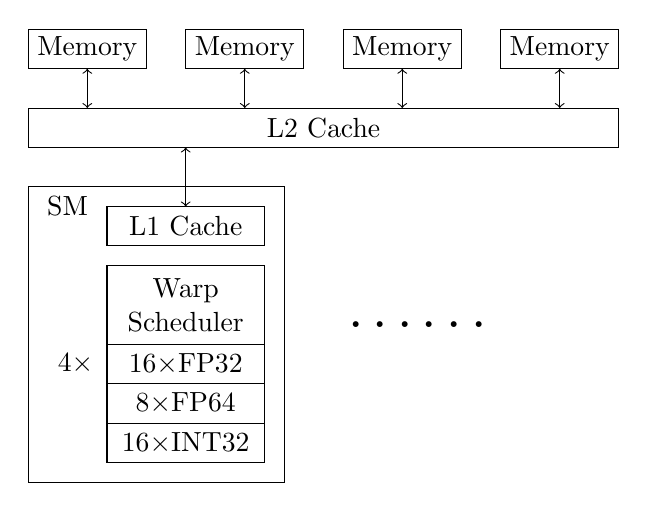
\begin{tikzpicture} 
        \foreach \x in {0,1,2,3} {
            \draw (\x*2, 0) rectangle +(1.5, 0.5) node[pos=.5] {Memory};
            \draw[<->] (\x*2+0.75, 0) -- +(0, -0.5);
        }
        \draw (0, -1) rectangle +(7.5, 0.5) node[pos=.5] {L2 Cache};

        \draw[<->] (2, -1) -- +(0, -0.75);

        \draw (0, -1.5) rectangle +(3.25, -3.75);
        \draw (1, -1.75) rectangle +(2, -0.5) node[pos=.5] {L1 Cache};
        
        \pic [local bounding box=sm_warp] at (1, -2.5) {sm_warp};
        \node[left of=sm_warp, xshift=-4mm] {$4\times$};
        \node at (0.5, -1.75) {SM};
        \node[scale=2] at (5, -3.25)  {\dots\dots};
    \end{tikzpicture}
    \caption{
        An overview of the memory hierarchy of the Ampere architecture. The L1 Cache is local to the SM which executes can 4 warps simultaneously 
    }
    \label{fig:ampere_architecture}
\end{figure}

Aside from the L1 and L2 caches, GPUs also use a translation lookaside buffer (TLB) which caches recent translations from virtual address space to physical address space.
\TODO{Explain virtual vs physical memory space}

\subsection{GPU Caches}
\label{sec:cache_gpu}
To the programmer, the memory hierarchy is very simplified: there is the compute unit and the memory.
Caches are hidden from this model as on most architectures they are managed by hardware.

Memory can become a significant bottleneck due to the large amount of threads running concurrently and the amount of data each thread processes.
Caches are much faster than memory and are often on the same chip as the compute unit.
However, they are limited in size, and a large enough problem can cause cache trashing -- the premature eviction of data before any significant reuse \cite{dai2016model}.
To improve the efficiency of caches, caches asume spatial locality via cache lines.
A cache line is the smallest unit of data that a cache can hold, and fetching data from memory also brings extra nearby data with it.
The L1 cache on a Turing GPU (and most other modern architectures) uses 128 byte cachelines which plays well with the 32-thread warp size since executing a fetch for a single precision floating point takes $32 \times 4 = 128$ bytes which can fit in a single cache line.
Data shared between threads through the cache can happen in a read-after-write (RAW) or read-after-read (RAR) manner.
RAW has data dependency between tasks, for example in scan operations.
RAR has no data dependency and can be executed in any order \cite{tripathy2021paver}.

The L1 cache in older Nvidia GPU architectures (Maxwell, Pascal) uses the least recently used (LRU) eviction policy.
When caches become full, we need to remove data (a cache line) from the cache to allow newer data to be cached.
An LRU eviction policy evicts data that is the least recently used.
\citet{mei2016dissecting} presented a novel fine-grained pointer chasing (P-chase) microbenchmark to explore unknown GPU cache parameters.
P-chase defines an array of indices where each element points to the next index to fetch from the array, thus chasing the pointer.

\citet{jia2019dissecting} have shown that in Turing and Volta GPUs, the P-chase benchmark that is used to detect the LRU eviction policy presented by \citet{mei2016dissecting} fails to complete over the full L1 cache.
\citeauthor{jia2019dissecting} conclude that newer architectures (Turing, Volta) uses a non-LRU eviction policy \cite{jia2019dissecting, jia2018dissecting,mei2016dissecting}.
When the L1 cache in Turing and Volta GPU saturates, 4 consecutive cache lines are chosen randomly to be evicted.
This is in line with a new eviction policy mechanism introduced with Volta, where cache lines can be assigned a priority \cite{jia2019dissecting,nvidia2021cudadocs}.

On the Turing architecture \citeauthor{jia2019dissecting} has found with the P-chase benchmark that the memory access latancy for a L2 cache miss and TLB miss to be 616 cycles.
On a L1 cache hit (best case scenario) the latency is 32 cycles.
For a L2 cache hit this rises to a latency of 188 cycles.
With L2 miss but a TLB hit the latency becomes 296 cycles.

Modern Nvidia GPUs are able to handle various types cache operations and eviction hints.
By default, loads are cached at all levels (L2, L1) with an LRU policy.
This brings a problem with it: if data is writen to a cached value, we need to evict this cache line from all other L1 caches first, since that value is no longer up to date after our update.
As an example, it is also possible to only cache on L2, bypassing L1.
Another option is to hint cache streaming, where the loaded cache line will have an evict-first policy to prevent polution of the cache.
Similar operations exist for writing data to memory.
In both cases it is up to the compiler and programmer to exploit this for extra performance \cite{nvidia2021cudadocs}.


\begin{table}
    \centering
    \begin{tabular}{l l l|r r r r}
        & Architecture & &    Turing &      Volta & Pascal & Maxwell
        \\
        & GPU Board    & &        T4 &       V100 &   P100 &     M60
        \\
        & GPU Chip     & &     TU104 &      GV100 &  GP100 &   GM204
        \\
        & Year         & &      2018 &       2017 &   2016 &    2014
        \\
        \hline
        L1 Cache%
        & Size     & KiB &  32 or 64 & 32\dots128 &     24 &      24
        \\
        & Line size  & B &        32 &         32 &     32 &      32
        \\
        \hline
        L2 Cache%
        & Size     & KiB &      4096 &      6144 &   4096 &    2048
        \\
        & Line size  & B &        64 &        64 &     32 &      32
        \\
        \hline
        L1 TLB%
        & Coverage   & MiB &      32 &        32 &   \~32 &     \~2
        \\
        & Page entry & KiB &    2048 &    2048   &   2048 &     128
        \\
        \hline
        L2 TLB%
        & Coverage   & MiB &  \~8192 &  \~8192   & \~2048 &   \~128
        \\
        & Page entry & MiB &      32 &      32   &     32 &       2
    \end{tabular}
    \caption{
        Summary of the cache specification on various Nvidia GPUs and architectures. 
        Adapted from \citeauthor{jia2019dissecting}\cite{jia2019dissecting}.
    }
\end{table}

\subsection{Kernel Execution}
\label{sec:kernel_execution}
When working with CUDA the programmer defines a kernel.
This is normally done with CUDA C++, an extension on C++ programming language, but in our case Accelerate will handle the generation of kernels (section \ref{sec:accelerate}) \cite{nvidia2021cudadocs}.

Executions on a GPU are directed on both the host and device (GPU).
\textit{Kernels} define the functions that should be executed on the GPU.
The host side controls how these kernels should be executed, namely how the threads should be launched and executed.
Threads are grouped and defined on a 2 level hierarchy: threads are grouped together in \textit{cooperative thread arrays} (CTAs), also known as thread blocks, and multiple CTAs can be queued for the execution of a single kernel.
Both can be controlled upon executing a kernel: the amount of threads per CTA (threadblock size) and the total amount of CTAs (gridsize).
CTAs get assigned to SMs in an arbitrary manner.

When an SM executes a CTA, it splits the work into warps, a grouping of 32-threads.
On architecture before Volta, a single warp is executed in a single instruction, multiple threads fashion, where a single program counter is shared amongst the 32 threads.
With the volta architecture, independent thread scheduling allows full concurency between threads and the scheduler can group multiple threads into SIMT units.

\TODO{SM can context switch between multipel warps to hide latency}

\TODO{Figure visualizing the whole thing because text is confusing... probably}

% random sketch
%\begin{figure}[!hb]
%    \centering
%    \begin{tikzpicture}
%        \pic at (0, 0) {thread};
%        \pic at (2, 0) {threadblock};
%        \pic at (5, 0) {warp};
%    \end{tikzpicture}
%    \caption{
%        \TODO{remove this, only used to debug tikz pic codes}
%    }
%\end{figure}


\begin{figure}[!hb]
    \centering
    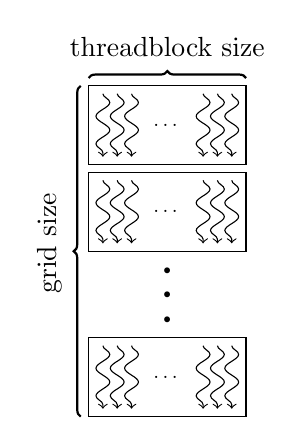
\begin{tikzpicture}
        \node at (1, 1.5) {threadblock size};
        \draw[decorate, thick, decoration={brace}] (0,1.1) --  (2,1.1);
        

        \node [rotate=90] at (-0.5, -1) {grid size};
        \draw[decorate, thick, decoration={brace}] (-0.1,-3.2) --  (-0.1,1);

        \pic at (0, 0) {threadblock};
        \pic at (0, -1.1) {threadblock};
        
        \node[scale=2, rotate=90] at (1, -1.6)  {\dots};
        \pic at (0, -3.2) {threadblock};
    \end{tikzpicture}
    \caption{
        GPU workloads are defined by the threadblock size and grid size.
    }
\end{figure}

\subsection{Performance of Access Patterns}
\citeauthor{lam1991cache} and \citeauthor{meyer2003algorithms} describe two types of reference reuse \cite{lam1991cache, meyer2003algorithms}:
\begin{itemize}
    \item \textbf{Spatial reuse} occurs when accessing data from the same cache line, increasing spatial locality.
    \item \textbf{Temporal reuse} occurs when the same data is accessed at a later time, increasing temporal locality.
\end{itemize}
The reuse factor can be kept track of by counting the two types of reuse.
Loading data horizontally (sequentially) exploits spatial locality and is therefore cheaper than loading data vertically.
Additionally, temporal reuse can only happen when other memory accesses do not displace reusable data from the cache.

\citeauthor{lam1991cache} proposed a method to model cache interference.
In the simplest case where all data used is cached in different locations (and therefore no data is evicted), the number of misses per variable $v$ is described by $D(v)/R(v)$, where $D(v)$ is the total number of references (loads) of $v$ and $R(v)$ is the reuse factor.
However, with interference misses when data gets displaced from cache, the total number of misses for $v$ is
\[
    D(v)\left(\frac{1}{R(v)}+\frac{R(v)-1}{R(v)}M(v)\right)
\]

With missrate being
\[
    M(v) = 1 \left(1 - S(v)\right) \prod_{u\in V - \{v\}}\left(1 - F(u)\right)
\]
$F(u)$ is defined as the fraction of cache used by variable $u$, and self interference $S(v)$ is defined to be the fraction of accesses that map to non-unique location in the cache.
In the context of blocking, the largest block size where no self-interference occurs is called the critical blocking factor.
From \citeauthor{lam1991cache}'s observations with matrix multiplications, the total amount of cache misses gradually declines with larger block sizes until the critical blocking factor is reached.

\TODO{Illustrations for interference}


\section{CPU vs GPU based multi-threading}
CPUs and GPUs differ in multiple ways.
GPUs consist out of many more cores compared to CPUs, however this also comes in a reduction in core complexity and capability.
In contrast, CPUs can leverage specialized instructions.
For example, Streaming SIMD Extensions (SSE) and Advanced Vector Extensions (AVX, AVX2, and AVX-512) allows CPU to process multiple data with singular instructions.
SSE can handle four 32-bit single-precision floating point numbers while AVX and AVX2 handle eight.
AVX-512 can handle sixteen, but is not widely implemented.

Caches also share the same hierarchical structure as the cores, however this differs per manufacturer and architecture.
Often the cache L1 is local to each thread, and L2 local to each core with 2 threads per core.

\section{Accelerate}
\TODO{Generalize to Array DSLs}
\label{sec:accelerate}
Accelerate is an embedded purely functional array language in Haskell \cite{chakravarty2011accelerating}.
Accelerate has a frontend containing the embedded language, and the backend which handles code generation and execution.
The frontend handles general optimizations such as sharing recovery and array fusion \cite{mcdonell2013optimising,balen2020optimal}.
Further hardware specific optimization is handled on the various backends.
There are two LLVM \cite{llvm} backends provided: one that targets multicore CPUs \texttt{accelerate-llvm-native} and one that targets Nvidia GPUs \texttt{accelerate-llvm-ptx}.
In both backends we compile Accelerate code to LLVM IR.
When we want to run Accelerate on a GPU, LLVM will handle the compilation from LLVM IR to PTX, the instructions set for Nvidia's CUDA programming environment \cite{mcdonell2015type, llvm, nvidia2021cudadocs}.
The GPU backend implements a series of skeletons which implement primitive operations such as stencils, generate, permute, and scan.
These skeletons define how a program should be compiled and is the part where a custom thread scheduler can be implemented.
Further customizations to the scheduler can be done on the executing side of the backend as it controls how kernels are launched.

\section{Commonly Applicable Cache Improvements}

\subsection{Optimizations of Blocked Algorithms}
\label{sec:optimization_blocked}
\citeauthor{lam1991cache} expands on the well known idea of working on blocks instead of entire rows or columns.

If all data fits onto cache without eviction, the misses that occur are \textit{intrinsic misses}.
In the real world however, data can be evicted by other memory accesses.
This interference of reuse is categorized between two cases: \textit{cross interference} and \textit{self interference}.
Cross interference assumes the location of data in memory is unrelated to the location in cache, and instead is measured by probablity that the reuse falls within the footprint of the variable.
Self interference extends this by taking the cache locations of variables into account, which can happen when the data for a single iteration no longer fits in cache.
\cite{lam1991cache}

\subsection{CTA Clustering}
\citeauthor{li2017locality} presented a clustering algorithm for reorder threads to improve cache performance on GPU.
It replaces a kernel with a new one with predefined clustering rules.
CTAs with inter-CTA locality are clustered together which can then be assigned to SMs.
The work in these clusters can be bounded to SMs in two ways:
Round-Robin Binding which asumes the scheduler assigns CTAs to SMs in a strict Round Robin policy, and SM-based binding which extracts the current executing SM for a CTA which it uses to devide the work it will do.
The former results in redirection based clustering while the latter forms agent based clustering.

Additionally, \citeauthor{li2017locality} implemented three optimizations into their clustering framework: 
\textbf{i) CTA Throttling} which limits the number of concurrent CTAs on an SM to reduce resource contention.
\textbf{ii) Cache Bypassing} to avoid unnecessary cache pollution.
\textbf{iii) CTA Prefetching using Reshaped Order}

CTA clustering observed no significant speedup for normal and dense matrix multiplications.
For convolutional neural networks (similar memory access patterns as stencils), a $1.4\times$ speedup was observed for redirection based clustering, and a $1.2\times$ speedup for other clustering algorithms of the Fermi architecture.
However, on the Pascal architecture, convolutional neural networks no speedup was observed, and on Maxwell and Kepler this improvement is limited to $1.1\times$.

\subsection{PAVER}
PAVER is very cool agent based clustering algorithm
\TODO{wRITE}

\chapter{Analysis of Existing Approaches}
\section{Assumptions}
During the analysis, we will asume a cache with an LRU eviction policy.
Additionally, we will not take into consideration cache associativity to simplify the analysis.

\section{Spatial Temporal Analysis}
\label{sec:st_analysis}
The memory accesses of an algorithm can be plotted in a spatial-temporal diagram, with the address space on the spatial axis and order of access on the temporal axis.
Since only the thread order can be manipulated, we do not need the granuality of the individual memory accesses within a thread.
This also avoids the problem of threads being concurrent and puts the focus on the temporal locaity between threads.
A different thread order shuffles the columns within this diagram: the same data is accessed but simply in a different order.

Additionally, we annotate this diagram with the cache level (L1, L2, RAM) of each memory address by simulating memory.
For the simulation we will use a simple LRU eviction policy which most Nvidia GPUs use and is similar to newer variation on the newer architectures like Turing and Volta, (see section \ref{sec:cache_gpu}).
\TODO{Feedback: do I need a smaller example?}

The resulting spatial temporal diagram (for example, figure \ref{fig:st_stencil_naive}) has the vertical axis describing the location in a 2D array which is mapped to 1D address space and the horizontal axis describing time. \fsquare{red} are addresses of cache lines that are brought into cache. \fsquare{black} are addresses being accessed. \fsquare{gray} are addresses in cache.

\section{Stencil Operations}

Stencil operation produces an N-dimensional array from a same sized input.
It consists of $I_w \times I_h$ tasks with $I_w$ being the first dimension of the input and $I_h$ being the product over the other dimensions.
For each element it reads a fixed sized $S_w \times S_h$ neighborhood and writes a single element.
Stencils are used for image operations (edge detection, filters, noise reduction), but can also find their use in other fields such as approximating partial differentiation\cite{roth1997compilingstencils} and cellular automata.
For example, a 2-dimensional $5 \times 5$ box blur filter over an input matrix $A$ can be mathemathically defined as:

\begin{equation}
    \texttt{Stencil}(x, y) = %
        \sum_{i=-2}^{2} %
        \sum_{j=-2}^{2} %
        \frac{ A[x + i, y + j] }{25}
    \label{eq:stencil_boxblur}
\end{equation}

In Accelerate, stencils are defined as listing \ref{lst:stencil_signature}, where the stencil function \texttt{stencil -> Exp b} takes in an N-dimensional tuple to produce a single value.
The boundary condition handles how boundary values are handled, either as a predefined function such as \texttt{clamp} and \texttt{mirror}, or as a user defined function.

\begin{listing}[H]
    \begin{minted}{haskell}    
stencil :: forall sh stencil a b. (Stencil sh a stencil, Elt b)	 
    -- stencil function
    => (stencil -> Exp b)
    -- boundary condition
    -> Boundary (Array sh a)	
    -- source array
    -> Acc (Array sh a)	
    -- destination array
    -> Acc (Array sh b)	
    \end{minted}
    \caption{
        The type signature of the stenciling function in Accelerate.
    }
    \label{lst:stencil_signature}
\end{listing}

To implement equation \ref{eq:stencil_boxblur} in Accelerate, we define a function to sum and divide all elements (listing \ref{lst:stencil_usuage}).

\begin{listing}[H]
    \begin{minted}{haskell}
-- Stencil types: included in Data.Array.Accelerate
type Stencil5 a = (Exp a, Exp a, Exp a, Exp a, Exp a) 
type Stencil5x5 a = (Stencil5 a, Stencil5 a, Stencil5 a, Stencil5 a, Stencil5 a) 

-- Example of a 5x5 box blurring stencil filter
boxblur5x5 :: Acc (Matrix Float) -> Acc (Matrix Float)
boxblur5x5 = A.stencil s A.clamp
  where
    -- Take a 5x5 array, then select each element and concatenate them
    s :: Stencil5x5 Float -> Exp Float
    s = average . concatMap (^..each) . (^..each)

    -- average all the elements in a list
    average :: Fractional a => [a] -> a
    average xs = sum xs / genericLength xs
    \end{minted}
    \caption{
        How to use the accelerate stenciling function (listing \ref{lst:stencil_signature}) to produce a $5 \times 5$ box blur filter.
    }
    \label{lst:stencil_usuage}
\end{listing}

\subsection{Naive}
\label{sec:stencil_naive}
The naive implementation iterates over each of the outputs linearly, horizontally first.
The temporal linearity translates to parallelism on GPUs where multiple threads work concurrently on each element of the output array.
The naive implementation of the $5 \times 5$ box blur filter (equation \ref{eq:stencil_boxblur} and listing \ref{lst:stencil_usuage}) is compareable to the following naive CUDA C++ implementation (listing \ref{lst:stencil_cuda}).

\begin{listing}[h]
    \begin{minted}{cuda}
#define STENCIL_SIZE 5

__global__ void stencil_naive(float *output, float *input, int width, int height, int N) {
    int tid = blockIdx.x * blockDim.x + threadIdx.x;
    int x = tid % width;
    int y = tid / width;
    
    if (tid >= N) {
        return;
    }

    float result = 0;
    for (int d_i = -STENCIL_SIZE/2; d_i <= STENCIL_SIZE/2; d_i++) {
        int i = min(height-1, max(0, y + d_i));
        for (int d_j = -STENCIL_SIZE/2; d_j <= STENCIL_SIZE/2; d_j++) {
            int j = min(width-1, max(0, x + d_j));
            result += input[i * width + j];
        }
    }
    output[tid] = result / (STENCIL_SIZE * STENCIL_SIZE);
}
    \end{minted}
    \caption{
        The naive CUDA C++ equivelant to listing \ref{lst:stencil_usuage}
    }
    \label{lst:stencil_cuda}
\end{listing}

While the naive implementation of stencil operations works well enough when enough rows of the input fit in the cache, it begins to fall in performance on larger inputs.
More specifically, inputs that are horizontally wide.

\begin{table}[h]
    \centering
    \begin{tabular}{|c c|}
        \hline
        Cache lines      & 24   \\
        Cache line width & 4    \\
        Eviction policy  & LRU  \\
        \hline
        Stencil size     & 7x7  \\
        Input Size       & 16x16\\
        Column size      & 8    \\
        \hline
    \end{tabular}
    \caption{
        The input parameters to generate the spatial-temporal diagrams for stencil operations.
    }
    \label{tab:sim_stencil_params}
\end{table}

% fig:st_stencil
\begin{figure}[H]
    \centering
    \subfloat[On input sizes too wide (i.e. $16 \times 16$) cache trashing occurs.]{
        \begin{tikzpicture}
            \node (image) at (0,0) {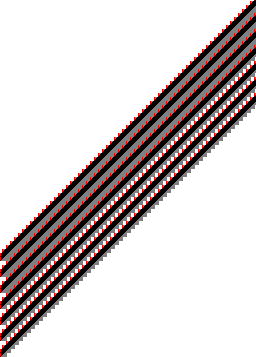
\includegraphics[width=0.4\textwidth]{st_diagrams/stencil7x7_linear.png}};
            \draw [->] (image.south west) -- ++(2,0) node[right]{\footnotesize\textit{Time}};
            \draw [->] (image.south west) -- ++(0,2) node[rotate=90, above]{\footnotesize\textit{Address}};
        \end{tikzpicture}
    }
    \qquad
    \subfloat[The input size is modified to $8 \times 32$ which results in optimal cache utilization.]{
        \begin{tikzpicture}
            \node (image) at (0,0) {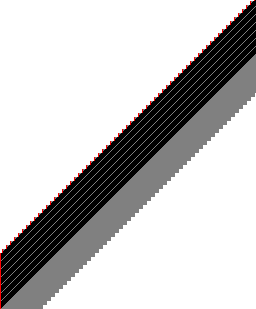
\includegraphics[width=0.4\textwidth]{st_diagrams/stencil7x7_linear_smaller_input.png}};
            \draw [->] (image.south west) -- ++(2,0) node[right]{\footnotesize\textit{Time}};
            \draw [->] (image.south west) -- ++(0,2) node[rotate=90, above]{\footnotesize\textit{Address}};
        \end{tikzpicture}
    }
    \caption{
        The spatial temporal diagram of a 7x7 stencil with linear ordering.
        See section \ref{sec:st_analysis}.
    }
    \label{fig:st_stencil_naive}
\end{figure}

% fig:stencil_naive_loading_pattern
\begin{figure}[!hb]
    \centering
    
    \subfloat[Ideal cache size, only minimal amount of loading is required.]{
        \centering
        \makebox[0.4\columnwidth][c]{
            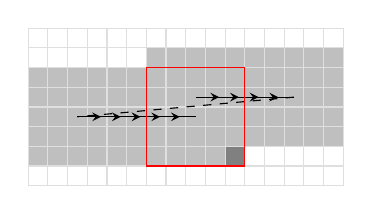
\begin{tikzpicture}[scale=0.25, decoration = {
                markings, mark = between positions 0.3cm and 0.95 step 0.25cm with {\arrow{stealth}}
            }]
                \fill[gray!50]  ( 6, 6) rectangle +(10, 1);
                \fill[gray!50]  ( 0, 2) rectangle +(16, 4);
                \fill[gray!50]  ( 0, 1) rectangle +(10, 1);
                \fill[gray!100] (10, 1) rectangle +( 1, 1);

                \draw[step=1,gray!25] (0, 0) grid (16, 8);
                \draw[black, postaction = decorate] (8.5, 4.5) -- +(5, 0);
                \draw[black, dashed] (13.5, 4.5) -- (2.5, 3.5);
                \draw[black, postaction = decorate] (2.5, 3.5) -- +(6, 0);
                \draw[red] (6,1) rectangle +(5, 5);
            \end{tikzpicture}
        }
        \label{fig:stencil_naive_loading_pattern_ideal}
    }
    \qquad
    \subfloat[Cache too small, data gets evicted before any potential reuse.]{
        \centering
        \makebox[0.4\columnwidth][c]{
            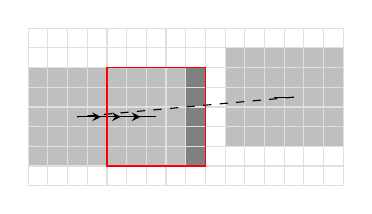
\begin{tikzpicture}[scale=0.25, decoration = {
                markings, mark = between positions 0.3cm and 0.95 step 0.25cm with {\arrow{stealth}}
            }]
                \fill[gray!50]  (10, 2) rectangle +( 6, 5);
                \fill[gray!50]  ( 0, 1) rectangle +( 8, 5);
                \fill[gray!100] ( 8, 1) rectangle +( 1, 5);

                \draw[step=1,gray!25] (0, 0) grid (16, 8);
                \draw[black, postaction = decorate] (12.5, 4.5) -- +(1, 0);
                \draw[black, dashed] (13.5, 4.5) -- (2.5, 3.5);
                \draw[black, postaction = decorate] (2.5, 3.5) -- +(4, 0);
                \draw[red] (4,1) rectangle +(5, 5);
            \end{tikzpicture}
        }
    }
    \caption{
        \TODO{write this}
    }
    \label{fig:stencil_naive_loading_pattern}
\end{figure}

The lower bound of cache in amount of cache lines needed $M_l$ is bounded by the total horizontal footprint $I_w + S_w$ in amount of cache lines $L$, multiplied by the stencil height $S_h$
\TODO{Maths}

\begin{equation}
    M_l \geq \ceil{\frac{I_w + S_w}{L}} S_h \label{eq:stencil_naive_optimal_memory}
\end{equation}

While in most cases \TODO{examples} this enough to fully exploit L2 caches, this can be unoptimal in regard to the L1 cache.
\TODO{Example}
The amount of cache lines needed to be fetched from memory $F$ is bound by the worse case (eq. \ref{eq:stencil_naive_optimal_memory} is not satisfied) where we consistently evict data from cache before we can reuse:

\[
    F \leq \ceil{\frac{I_w + S_w}{L}} I_h S_h
\]

If equation \ref{eq:stencil_naive_optimal_memory} is satisfied, the amount of fetches $F$ is no longer depedent on the stencil height $S_h$

\[
    F = \ceil{\frac{I_w + S_w}{L}} I_h
\]

\TODO{GPU threading is different from CPU stuff yada yada}
With multiple threads active, even more data is required to be kept in cache for optimal usuage.
In the best case, all threads are cohesive with overlapping accesses, and in the worst case, threads will be spread out more with less overlapping accesses.
Threads in GPUs are grouped by warps, threads contained within are always cohered, and therefore a guarantee for overlapping accesses.
Therefore, only when multiple warps are executed on the same SM, divergence in accesses can occur.
A single warp of 32 threads uses $\ceil{\frac{32 + S_w}{l}} S_h$ cache lines when the threads cover a single rows. 
When the warp is split between 2 rows, the cache needs to be slightly bigger: $\ceil{\frac{32 + 2 S_w}{l}} S_h$.

Ideally, the whole input array would fit on the cache, but a sufficiently large input (e.g. a $2048\times2048$ 32-bit floating point array uses 16 MiB) will not fit on the L2 caches of modern GPUs ($\approx6$MiB of L2 data cache, Volta V100) and cache misses are unavoidable.
Even if data would fit on the L2 cache, there would still be potential cache misses at the L1 cache (128 KiB, Volta V100).

\TODO{More figures like in fig. \ref{fig:stencil_naive_loading_pattern}, but for GPU/multithreading}

\vspace{2cm}

Using the model described in section \ref{sec:cache_gpu} can be used to estimate the cache misses of the naive implementation and the model parameters are summarized in table \ref{tab:stencil_naive_model}.
Calculating the reuse for an iteration of $s_y$, $i_x$, and $i_y$ is fairly trivial.

\TODO{These are the calculations adapted from Lam et al. 1991. I'm not really sure if I should do this. They feel not very ellegant, and more like a black box system\dots}
$s_x$ is ommited due to it only loading a singular value during one loop and has therefore no reuse.
During a single step of $s_y$ an entire row of all $S_w$ elements from the stencil has been loaded.
A single step on $i_x$ processes the output of a singular element, which means an entire stencil is read.


\begin{table}[H]
    \centering
    \begin{tabular}{|c||c|c|c|c||c|c|c|c|}
        \hline
        Array & \multicolumn{4}{c||}{Reuse} & \multicolumn{4}{c|}{Self-Interference}
        \\ \hline
        & $i_x$ & $i_y$ & $s_x$ & $s_y$
        & $i_x$ & $i_y$ & $s_x$ & $s_y$
        \\ \hline
        X & $(S_w - 1)S_h$ & $(S_h - 1) S_w I_w$ & - & $S_w$
        & &  & 0 & 0

        \\ \hhline{*{9}{=}}
        Array & \multicolumn{4}{c||}{Footprint} &  \multicolumn{4}{c|}{References}
        \\ \hline
        & $i_x$ & $i_y$ & $s_x$ & $s_y$ & \multicolumn{4}{c|}{}
        \\ \hline
        X & $S_wS_h/C$ & $I_wS_h/C$ & $1/C$ & $S_w/C$ &
        \multicolumn{4}{c|}{$I_w I_h S_w S_h$}
        \\ \hline
    \end{tabular}

    \caption{
        The reuse, self-interference, and footprint of the naive implementation of stencils during a single step of iterating on $i_x$, $i_y$, $s_x$, and $s_y$.
        \TODO{Calculate self interference}
    }
    \label{tab:stencil_naive_model}
\end{table}

\subsection{Tiling}
\label{sec:stencil_tiled}
A common used optimization is by dividing the work into works as described in \ref{sec:optimization_blocked}.
\TODO{blablablabla}

The minimum required cache for optimal tiling is depedent on \TODO{\dots} tiling size $t$

\begin{equation}
    M_l \geq \ceil{\frac{t + S_w}{L}} S_h \label{eq:stencil_tiling_memory}
\end{equation}

The largest possible tiling size $t$ is derived by inverting equation \ref{eq:stencil_tiling_memory}

\begin{equation}
    t \leq \frac{L M_l}{S_h} - S_w
\end{equation}

In practise, equation \ref{eq:stencil_tiling_memory} can be satisfied by adjusting $t$, we can have a lower upper bound on the amount of cache line fetches $F$:

\begin{equation}
    F \leq \ceil{\frac{I_w}{t}} \ceil{\frac{t + S_w}{L}} \ceil{\frac{I_h}{t}} (t + S_h)
    \label{eq:stencil_tiling_fetches}
\end{equation}

\TODO{Maybe remove this. Probably just keep it, so we can plot our expected number of cache line fetches}
We can define the number cache lines fetched in terms of the available cache by substituting equation \ref{eq:stencil_tiling_memory} into equation \ref{eq:stencil_tiling_fetches}:

\begin{equation}
    F \leq \ceil{\frac{I_w}{\frac{L M_l}{S_h} - S_w}} \ceil{\frac{\frac{L M_l}{S_h} - S_w + S_w}{L}} \ceil{\frac{I_h}{\frac{L M_l}{S_h} - S_w}} \left(\frac{L M_l}{S_h} - S_w + S_h\right)
\end{equation}

\begin{equation}
    F \leq \frac{I_w I_h M_l}{(\frac{L M_l}{S_h} - S_w)^2 S_h} (\frac{L M_l}{S_h} - S_w + S_h)
\end{equation}
\TODO{simplify this further by relaxation perhaps?}


\TODO{GPU/multithreading notes}

\section{Matrix Multiplication}

\subsection{Naive}
\TODO{writewrite}
\begin{listing}[H]
    \begin{minted}{cuda}
__global__ void matrix_naive(float *o, float *a, float *b, int depth, int width, int height) {
    int tid = blockIdx.x * blockDim.x + threadIdx.x;
    int x = tid % width;
    int y = tid / width;
    
    if (tid >= width * height) {
        return;
    }

    float result = 0;
    for (int i = 0; i < depth; i++) {
        result += a[y * depth + i] * b[x + i * width];
    }
    o[tid] = result;
    
}
    \end{minted}
    \caption{
        The naive CUDA C++ implementation of matrix multiplication
    }
    \label{lst:mm_naive_cuda}
\end{listing}

\begin{table}[H]
    \centering
    \begin{tabular}{|c c|}
        \hline
        Cache lines      & 32   \\
        Cache line width & 4    \\
        Eviction policy  & LRU  \\
        \hline
        Input Size       & 16x16\\
        Column size      & 8    \\
        \hline
    \end{tabular}
    \caption{
        The input parameters to generate the spatial-temporal diagrams for matrix multiplications.
    }
    \label{tab:sim_matrix_params}
\end{table}

% fig:st_matrix
\begin{figure}[H]
    \centering
    \begin{tikzpicture}[spy using outlines={rectangle, magnification=4,connect spies}]
        \node (image) at (0,0) {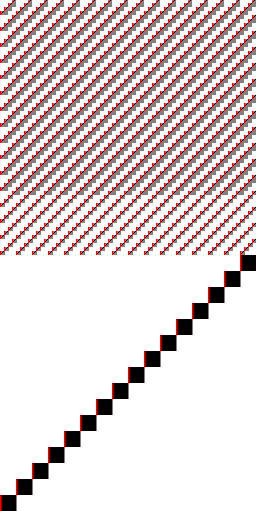
\includegraphics[width=0.25\textwidth]{st_diagrams/matrix_linear.png}};
        \draw [->] (image.south west) -- ++(2,0) node[right]{\footnotesize\textit{Time}};
        \draw [->] (image.south west) -- ++(0,8.5) node[rotate=90, above left]{\footnotesize\textit{Memory Addresses}};

        \coordinate (p) at (0, 1);
        \coordinate (v) at (3.3, 2);
        \spy[width=2.4cm,height=4cm] on (p) in node [fill=white] at (v);
    \end{tikzpicture}

    \caption{
        The spatial temporal diagram of matrix multiplication with linear ordering. 
        See section \ref{sec:st_analysis}.
    }
    \label{fig:st_matrix_naive}
\end{figure}

Given the output matrix $C$ of size $I_w \times I_h$ with input matrices $A$ and $B$ of size $I_w \times D$ and $D \times I_h$ respectively, data from $B$ can be reused in the naive case only if we can both keep one row of $B$ and one column of $A$ loaded.

\begin{equation}
    \label{eq:mm_naive_minimum_cache}
    M_l > \ceil{\frac{D}{L}} + D
\end{equation}

\noindent
If equation \ref{eq:mm_naive_minimum_cache} is satisfied, the amount of cacheloads is roughly

\begin{equation}
    F \approx \ceil{\frac{D}{L}} I_h + D I_w I_h
\end{equation}

\noindent
In the case that equation \ref{eq:mm_naive_minimum_cache} is not satisfied, there is no reuse of data possible, and the amount of cache line fetches is

\begin{equation}
    F \approx \left( \ceil{\frac{D}{L}} + D \right) I_w I_h
\end{equation}

\noindent
To reuse date from both matrix $A$ and $B$ requires to keep the entirity of $A$ cached until we work on the second row.

\begin{equation}
    M_l > \ceil{\frac{D}{L}} + \ceil{\frac{I_w D}{L}}
\end{equation}

\noindent
This lowers the amount of cache loads significantly

\begin{equation}
    F \approx \ceil{\frac{D}{L}} I_h + \ceil{\frac{I_w}{L}} D
\end{equation}

\subsection{Tiling}
Tiling is a common optimization technique for matrix multiplication.
\citet{lam1991cache} suggests a blocking factor of $\sqrt{C/2}$ since at that point selft interference is minimum.

\subsection{(S)GEMM in cuBLAS}
(Single) Precision General Matrix Multiplication (SGEMM) in Nvidia's implementation of Basic Linear Algebra Subroutines (BLAS) named cuBLAS is a closed sourced library that implements a very optimized GPU based matrix multiplication.


\chapter{Column Based Iteration}
While tiling itself is a well-known optimization technique, we must consider the parts of why it works.
Temporal locality is increased because the scope of the work is smaller, which is done by sacraficing a bit of spatial locality: we no longer load an entire row, only a part.
However, this only explains the horizontal tiling, vertical tiling only reduces the scope as we work on a smaller tile but when considering the entire workload, it ultimately does not matter.
It can even be argued that by tiling vertically, we fragment the the workload as temporal locality cannot be guaranteed between tiles.

\section{Theory}
\label{sec:implementation_theory}

In a sense, grouping columns is similar to striding clusters of data, except in the case when a row of work can't be perfectly strided.
When the width of a multidimensional array is not a multiple of the stride, the loads will not align column wise (figure \ref{fig:column_vs_striding}).
To work around this, in the column approach we allow the last column to be narrower.

\begin{figure}[!hb]
    \centering
    
    \subfloat[Striding does not work well when the width of the task is a non-multiple of the striding factor.]{
        \centering
        \makebox[0.4\columnwidth][c]{
            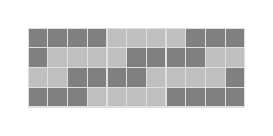
\begin{tikzpicture}[scale=0.25, decoration = {
                markings, mark = between positions 0.3cm and 0.95 step 0.25cm with {\arrow{stealth}}
            }]
                \fill[gray]    (0, 3) rectangle +(4, 1);
                \fill[gray!50] (4, 3) rectangle +(4, 1);
                \fill[gray]    (8, 3) rectangle +(3, 1);

                \fill[gray]    (0, 2) rectangle +(1, 1);
                \fill[gray!50] (1, 2) rectangle +(4, 1);
                \fill[gray]    (5, 2) rectangle +(4, 1);
                \fill[gray!50] (9, 2) rectangle +(2, 1);

                \fill[gray!50] (0, 1) rectangle +(2, 1);
                \fill[gray]    (2, 1) rectangle +(4, 1);
                \fill[gray!50] (6, 1) rectangle +(4, 1);
                \fill[gray]    (10, 1) rectangle +(1, 1);

                \fill[gray]    (0, 0) rectangle +(3, 1);
                \fill[gray!50] (3, 0) rectangle +(4, 1);
                \fill[gray]    (7, 0) rectangle +(4, 1);

                \draw[step=1,gray!25] (0, 0) grid (11, 4);
            \end{tikzpicture}
        }
        \label{fig:striding_misalignment}
    }
    \qquad
    \subfloat[Allowing the last column to be flexible allows columns of thread groups to stay cohesive.]{
        \centering
        \makebox[0.4\columnwidth][c]{
            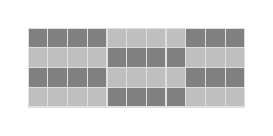
\begin{tikzpicture}[scale=0.25, decoration = {
                markings, mark = between positions 0.3cm and 0.95 step 0.25cm with {\arrow{stealth}}
            }]
                \fill[gray]    (0, 3) rectangle +(4, 1);
                \fill[gray!50] (4, 3) rectangle +(4, 1);
                \fill[gray]    (8, 3) rectangle +(3, 1);

                \fill[gray!50] (0, 2) rectangle +(4, 1);
                \fill[gray]    (4, 2) rectangle +(4, 1);
                \fill[gray!50] (8, 2) rectangle +(3, 1);

                \fill[gray]    (0, 1) rectangle +(4, 1);
                \fill[gray!50] (4, 1) rectangle +(4, 1);
                \fill[gray]    (8, 1) rectangle +(3, 1);

                \fill[gray!50] (0, 0) rectangle +(4, 1);
                \fill[gray]    (4, 0) rectangle +(4, 1);
                \fill[gray!50] (8, 0) rectangle +(3, 1);

                \draw[step=1,gray!25] (0, 0) grid (11, 4);
            \end{tikzpicture}
        }
        \label{fig:column_alignment}
    }
    \caption{
        Striding does not work if the stride does not fit perfectly in the input width. Flexibility is required.
    }
    \label{fig:column_vs_striding}
\end{figure}

\noindent
The index mapping $i \mapsto j$ to get the columning order consists out of four parts (figure \ref{fig:column_remap_parts}):
\begin{itemize}
    \item The starting offset of the column $o$.
    \item The column width $w'$.
    \item The index within a column $i'$.
    \item The position within the column $(x, y)$.
\end{itemize}

\begin{figure}[!hb]
    \centering
    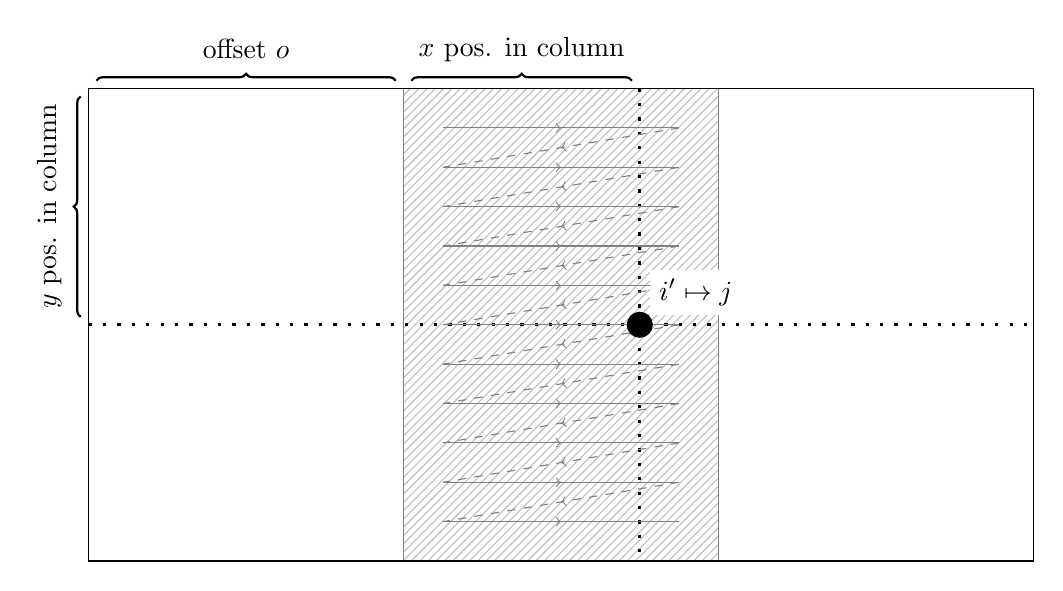
\begin{tikzpicture}
        % offset
        \node at (2, 0.5) {offset $o$};
        \draw[decorate, thick, decoration={brace}] (0.1,0.1) --  (3.9,0.1);

        % x
        \node at (5.5, 0.5) {$x$ pos. in column};
        \draw[decorate, thick, decoration={brace}] (4.1,0.1) --  (6.9,0.1);

        % y
        \node [rotate=90] at (-0.5, -1.5) {$y$ pos. in column};
        \draw[decorate, thick, decoration={brace}] (-0.1,-2.9) -- (-0.1,-0.1);

        % current column:
        \draw[gray, pattern=north east lines, pattern color=gray!50] (4,0) rectangle (8, -6);

        % input array:
        \draw (0, 0) rectangle (12, -6);

        \draw[loosely dotted, very thick] (7, 0) -- (7,-6);
        \draw[loosely dotted, very thick] (0, -3) -- (12,-3);

        \foreach \i in {0.5,1.0,...,5} {
            \draw[gray, ->-] (4.5,-\i) -- (7.5,-\i);
            \draw[gray, ->-, dashed] (7.5,-\i) -- (4.5,-\i - 0.5);
        }
        \draw[gray, ->-] (4.5,-5.5) -- (7.5,-5.5);
        
        \node[fill, circle, label={[fill=white]above right:$i' \mapsto j$}] at (7, -3) {};

    \end{tikzpicture}
    \caption{
        The anatomy of the column based index remapping.
    }
    \label{fig:column_remap_parts}
\end{figure}

First, we calculate the offset for the starting index of the column we need to map to:

\begin{align}
    o  &= \floor{\frac{i}{I_h w}} w
    \\ \intertext{Then, modify the width value such that the last column does not exceed the input width:}
    w' &= \begin{cases}
        I_w - o& \text{if last column}
        \\
        w & \text{otherwise}
    \end{cases}
    \\ \intertext{And take $i'$ as the index within a column:}
    i' &= i \bmod I_h w'
    \\ \intertext{Calculate the position $(x, y)$ within the column:}
    x & = i' \bmod w'
    \\ 
    y & = \floor{\frac{i'}{w'}}
    \\ \intertext{So that we can calculate $j$:}
    \label{eq:column_mapping_to_j}
    j  &= x + y I_w + o
\end{align}

On GPUs threads in threadblocks are batched in warps of 32 threads and these warps may be executed in an arbitrary order (section \ref{sec:kernel_execution}).
As a result we might not be able to exploit the cache as much since column orders are highly dependent on thread order and on the higher level, CTAs may be assigned in a completely arbitrary way.

\subsection{Zigzagging variation}
When working in warps of 32-threads and having a non-multiple of 32 wide columns, the workload for a warp may be spread out due to the tail end of our task being put at the beginning of the next row.
A solution to this may be to zigzag every other row such that when working on another row, our accesses are still local.
We can modify equation \ref{eq:column_mapping_to_j}:

\begin{equation}
    j = \left(\begin{cases}
        x & y \text{ is uneven}
        \\
        w' - x & y \text{ is even}
    \end{cases}\right)  + y I_w + o
\end{equation}

\subsection{Higher dimensions}
Since only work horizontally gets split, this algorithm may work on higher dimensions since in N-dimensional arrays, only one dimension can properly benefit from spatial locality.
All other dimensions can only exploit temporal locality.
We can therefore encapsulate an N-dimensional problem into 2-dimensional (horziontal and vertical) one, by mapping all but the first dimension to the vertical dimension.

\section{Implementation}

The remapping algorithm described in section \ref{sec:implementation_theory} can be directly transcribed into C code (listing \ref{lst:column_cuda}).
\begin{listing}[ht]
    \begin{minted}{cuda}
__global__ void my_kernel(int width, [...]){
    // For a given thread ID we can compute the 
    // new thread ID and it's x, y position:
    int tid = blockIdx.x * blockDim.x + threadIdx.x;
    int x; // originally x = tid % width;
    int y; // originally y = tid / width;

    if (tid >= width * height) {
        return;
    }

    int col_size = height * col_w;

    // Column identifier
    int col_id  = tid / col_size;

    // Thread id within column
    int col_tid = tid % col_size;

    // Column offset
    int col_off = col_id * col_w;

    // True width of column
    //
    // int col_tw  = col_w;
    // if (col_id == width  / col_w) {
    //     col_tw  = width - col_id * col_w;
    // }
    //
    // A shorter version of  the above since col_tw is 
    // always bounded by col_w. It removes the need of 
    // an expensive  divide operation  and saves 2 PTX
    // instructions overal. 
    
    int col_tw = min(width - col_id * col_w, col_w);

    x = (col_tid % col_tw) + col_off;
    y =  col_tid / col_tw;
    tid = x + (y * width);

    do_things_with(tid, x, y);
}
    \end{minted}
    \caption{
        The CUDA C++ implementation column based remapping.
    }
    \label{lst:column_cuda}
\end{listing}


\begin{listing}[ht]
    \begin{minted}{cuda}
__global__ void my_kernel(int col_w, int width, [...]){
    int tid = blockIdx.x * blockDim.x + threadIdx.x;
    int x; // originally x = tid % width;
    int y; // originally y = tid / width;

    int col_size = height * col_w;
    int col_id  = tid / col_size;
    int col_tid = tid % col_size;
    int col_off = col_id * col_w;
    int col_tw = min(width - col_id * col_w, col_w);

    x = (col_tid % col_tw) + col_off;
    y =  col_tid / col_tw;
    tid = x + (y * width);

    do_things_with(tid, x, y);
}
    \end{minted}
    \caption{
        The CUDA C++ implementation column based remapping.
    }
    \label{lst:column_cuda2}
\end{listing}

For the implementation in Accelerate, we first define the type signature of a thread id mapping function (listing {\ref{lst:threadmapping_type}}).
\begin{listing}[!ht]
    \begin{minted}{haskell}    
type ThreadMapping sh e arch 
    =  ShapeR sh 
    -> Operands sh 
    -> Operands Int 
    -> CodeGen arch (Operands Int)
    \end{minted}
    \caption{
        The type signature of a thread remapping function which takes the input dimension sizes and thread index and produces a new thread index.
    }
    \label{lst:threadmapping_type}
\end{listing}
We then implement the algorithm as described in section \ref{sec:implementation_theory} (listing \ref{lst:column_mapping})
\begin{listing}
    \begin{minted}{haskell}
column :: Operands Int -> ThreadMapping sh e arch
column column_width shr sh index = do
    -- input sizes
    input_width  <- widthOp shr sh
    input_size   <- sizeOp  shr sh
    input_height <- input_size |//| input_width
    
    column_size  <- column_width |*|  input_height
    column_count <- ((input_size |+| column_size) |-| (1::Int)) |//| column_size

    column_index      <- index |//| column_size
    column_last_index <- column_count |-| (1::Int)
    column_offset     <- column_index |*| column_width

    index' <- index |%| column_size

    column_current_width <- ifThenElse (
        TupRsingle $ SingleScalarType $ NumSingleType (numType @Int), 
        column_index |==| column_last_index
      ) ( do
        input_width |-| (column_last_index |*| column_width)
      ) ( do
        return column_width
      )
    
    x_in_column <- index' |%|  column_current_width
    y_in_column <- index' |//| column_current_width
    result      <- x_in_column |+| (y_in_column |*| input_width) |+| column_offset

    return result
    \end{minted}
    \caption{
        The thread remapping function for Accelerate implemented in Haskell.
    }
    \label{lst:column_mapping}
\end{listing}
However, in Accelerate a single thread can work on multiple elements if the work is larger than the maximum number of threads.
Instead of computing the complete remap every new index, we can precompute part of the algorithm (listing \ref{lst:column_mapping_precompute}).

\begin{listing}
    \begin{minted}{haskell}
precomp_column :: Operands Int 
               -> ShapeR sh 
               -> Operands sh 
               -> CodeGen arch (Operands Int -> CodeGen arch (Operands Int))
precomp_column column_width shr sh = do
    -- input sizes
    input_width  <- widthOp shr sh
    input_size   <- sizeOp  shr sh
    input_height <- input_size |//| input_width
    
    column_size  <- column_width |*|  input_height
    column_count <- ((input_size |+| column_size) |-| (1::Int)) |//| column_size

    column_last_index <- column_count |-| (1::Int)

    return \index -> do
        column_index  <- index |//| column_size
        column_offset <- column_index |*| column_width
        index' <- index |%| column_size

        column_current_width <- ifThenElse (
            TupRsingle $ SingleScalarType $ NumSingleType (numType @Int), 
            column_index |==| column_last_index
        ) ( do
            input_width |-| (column_last_index |*| column_width)
        ) ( do
            return column_width
        )
        
        x_in_column <- index' |%|  column_current_width
        y_in_column <- index' |//| column_current_width
        result      <- x_in_column |+| (y_in_column |*| input_width) |+| column_offset

        return result
    \end{minted}
    \caption{
        The column mapping from listing \ref{lst:column_mapping} with precomputing the fixed parameters.
    }
    \label{lst:column_mapping_precompute}
\end{listing}

\section{Stencil Operation}

The naive stencil operations had problems of chasing the cache on sufficiently large input sizes which tiling does resolve (section \ref{sec:stencil_tiled}).
Consider what the tiling implies: we split the work on all axis, to improve locality.
However, all tiling except horizontal is can be considered unnecessary because vertical tiling only causes to fragmentize the workload.

Let us first consider the single threaded case of column based iteration: by controlling the column width we can force the ideal scenario of the naive stencil implementation (figure \ref{fig:stencil_naive_loading_pattern_ideal}) to occur, similarly to tiling.
The column based approach is similar to tiling, but also allows the ideal memory access pattern to continue accross tiles vertically.
In GPUs this translates to less cohesive threads as threadblocks get assigned in a round-robin fashion to SMs, eliminating posibilities of L1 cache reuse.

\begin{figure}[!hb]
    \centering
    
    \subfloat[Grouping by column only incurs a heavy load every time a new column is started.]{
        \centering
        \makebox[0.4\columnwidth][c]{
            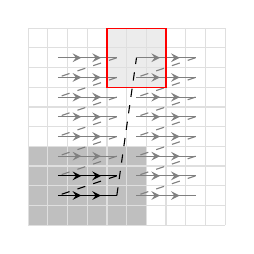
\begin{tikzpicture}[scale=0.25, decoration = {
                markings, mark = between positions 0.3cm and 0.95 step 0.25cm with {\arrow{stealth}}
            }]
                \fill[gray!50]  (-1, -1) rectangle +(6, 4);
                \fill[gray!15] (3, 6) rectangle +(3, 3);

                \draw[step=1,gray!25] (-1, -1) grid (9, 9);

                \draw[gray, postaction = decorate] (0.5, 7.5) -- +(3, 0);
                \draw[gray, dashed] (3.5, 7.5) -- +(-3, -1);
                \draw[gray, postaction = decorate] (0.5, 6.5) -- +(3, 0);
                \draw[gray, dashed] (3.5, 6.5) -- +(-3, -1);
                \draw[gray, postaction = decorate] (0.5, 5.5) -- +(3, 0);
                \draw[gray, dashed] (3.5, 5.5) -- +(-3, -1);
                \draw[gray, postaction = decorate] (0.5, 4.5) -- +(3, 0);
                \draw[gray, dashed] (3.5, 4.5) -- +(-3, -1);
                \draw[gray, postaction = decorate] (0.5, 3.5) -- +(3, 0);
                \draw[gray, dashed] (3.5, 3.5) -- +(-3, -1);
                \draw[gray, postaction = decorate] (0.5, 2.5) -- +(3, 0);
                \draw[gray, dashed] (3.5, 2.5) -- +(-3, -1);
                \draw[black, postaction = decorate] (0.5, 1.5) -- +(3, 0);
                \draw[black, dashed] (3.5, 1.5) -- +(-3, -1);
                \draw[black, postaction = decorate] (0.5, 0.5) -- +(3, 0);

                \draw[black, dashed] (3.5, 0.5) -- +(1, 7);
                
                \draw[gray, postaction = decorate] (4.5, 7.5) -- +(3, 0);
                \draw[gray, dashed] (7.5, 7.5) -- +(-3, -1);
                \draw[gray, postaction = decorate] (4.5, 6.5) -- +(3, 0);
                \draw[gray, dashed] (7.5, 6.5) -- +(-3, -1);
                \draw[gray, postaction = decorate] (4.5, 5.5) -- +(3, 0);
                \draw[gray, dashed] (7.5, 5.5) -- +(-3, -1);
                \draw[gray, postaction = decorate] (4.5, 4.5) -- +(3, 0);
                \draw[gray, dashed] (7.5, 4.5) -- +(-3, -1);
                \draw[gray, postaction = decorate] (4.5, 3.5) -- +(3, 0);
                \draw[gray, dashed] (7.5, 3.5) -- +(-3, -1);
                \draw[gray, postaction = decorate] (4.5, 2.5) -- +(3, 0);
                \draw[gray, dashed] (7.5, 2.5) -- +(-3, -1);
                \draw[gray, postaction = decorate] (4.5, 1.5) -- +(3, 0);
                \draw[gray, dashed] (7.5, 1.5) -- +(-3, -1);
                \draw[gray, postaction = decorate] (4.5, 0.5) -- +(3, 0);
                \draw[red] (3,6) rectangle +(3, 3);
            \end{tikzpicture}
        }
    }
    \label{fig:}
    \qquad
    \subfloat[Tiling also incurs a heavy load when starting a new row of tiles, and due to having more rows also has more column starts.]{
        \centering
        \makebox[0.4\columnwidth][c]{
            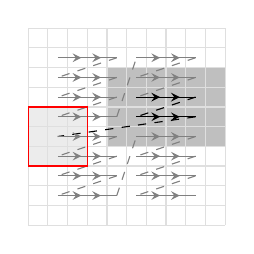
\begin{tikzpicture}[scale=0.25, decoration = {
                markings, mark = between positions 0.3cm and 0.95 step 0.25cm with {\arrow{stealth}}
            }]
            \fill[gray!50] (3, 3) rectangle +(6, 4);
            \fill[gray!15] (-1, 2) rectangle +(3, 3);

            \draw[step=1,gray!25] (-1, -1) grid (9, 9);

            \draw[gray, postaction = decorate] (0.5, 7.5) -- +(3, 0);
            \draw[gray, dashed] (3.5, 7.5) -- +(-3, -1);
            \draw[gray, postaction = decorate] (0.5, 6.5) -- +(3, 0);
            \draw[gray, dashed] (3.5, 6.5) -- +(-3, -1);
            \draw[gray, postaction = decorate] (0.5, 5.5) -- +(3, 0);
            \draw[gray, dashed] (3.5, 5.5) -- +(-3, -1);
            \draw[gray, postaction = decorate] (0.5, 4.5) -- +(3, 0);
            \draw[gray, dashed] (3.5, 4.5) -- +(1, 3);
            \draw[gray, postaction = decorate] (4.5, 7.5) -- +(3, 0);
            \draw[gray, dashed] (7.5, 7.5) -- +(-3, -1);
            \draw[gray, postaction = decorate] (4.5, 6.5) -- +(3, 0);
            \draw[gray, dashed] (7.5, 6.5) -- +(-3, -1);
            \draw[black, postaction = decorate] (4.5, 5.5) -- +(3, 0);
            \draw[black, dashed] (7.5, 5.5) -- +(-3, -1);
            \draw[black, postaction = decorate] (4.5, 4.5) -- +(3, 0);
            
            \draw[black, dashed] (7.5, 4.5) -- +(-7, -1);

            \draw[gray, postaction = decorate] (0.5, 3.5) -- +(3, 0);
            \draw[gray, dashed] (3.5, 3.5) -- +(-3, -1);
            \draw[gray, postaction = decorate] (0.5, 2.5) -- +(3, 0);
            \draw[gray, dashed] (3.5, 2.5) -- +(-3, -1);
            \draw[gray, postaction = decorate] (0.5, 1.5) -- +(3, 0);
            \draw[gray, dashed] (3.5, 1.5) -- +(-3, -1);
            \draw[gray, postaction = decorate] (0.5, 0.5) -- +(3, 0);
            \draw[gray, dashed] (3.5, 0.5) -- +(1, 3);
            \draw[gray, postaction = decorate] (4.5, 3.5) -- +(3, 0);
            \draw[gray, dashed] (7.5, 3.5) -- +(-3, -1);
            \draw[gray, postaction = decorate] (4.5, 2.5) -- +(3, 0);
            \draw[gray, dashed] (7.5, 2.5) -- +(-3, -1);
            \draw[gray, postaction = decorate] (4.5, 1.5) -- +(3, 0);
            \draw[gray, dashed] (7.5, 1.5) -- +(-3, -1);
            \draw[gray, postaction = decorate] (4.5, 0.5) -- +(3, 0);
            \draw[red] (-1,2) rectangle +(3, 3);
            \end{tikzpicture}
        }
    }
    \caption{
        Visualisation of cache bottlenecks for both column based and tiling approaches. 
        \fsquare{red} Memory required by the next task.
        \fsquare{black} Tasks that still have their memory in cache.
        \fsquare{gray!50} Memory in cache.
        \fsquare{gray!15} Previous and upcoming tasks.
    }
    \label{fig:stencil_column_vs_tiling_pattern}
\end{figure}

\begin{figure}
    \centering
    \begin{tikzpicture}
        \node (image) at (0,0) {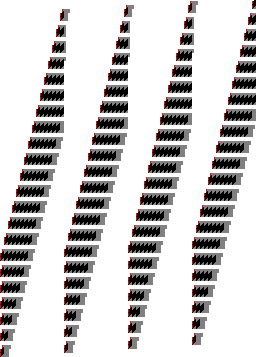
\includegraphics[width=0.4\textwidth]{st_diagrams/stencil7x7_column_4.png}};
        \draw [->] (image.south west) -- ++(2,0) node[right]{\footnotesize\textit{Time}};
        \draw [->] (image.south west) -- ++(0,2) node[rotate=90, above]{\footnotesize\textit{Address}};
    \end{tikzpicture}
    \caption{
        The spatial temporal diagram of a 7x7 stencil with a column of size 4 ordering.
        See section \ref{sec:st_analysis}.
    }
    \label{fig:st_stencil_column}
\end{figure}

The size of the cache needed $M_{size}$ can be approximated given the units per cache line $L$, column width $c$, stencil width $s_{w}$ and height $s_{h}$, and the number of active threads $t$. The required memory is independent of the size of the input data.

\[
    M_{size} = u \left(c + s_w\right) \left(s_h + \ceil{\frac{t}{c}}\right)
\]

Solving for $c$ gives an unneedly complex solution, so instead we approximate $M_{size}$ using the asymptote.

\[
    M_{size} = u \left(t + s_h \left(c + s_w\right)\right)
\]

Solving for column width $c$ gives 

\[
    c = \frac{M_{size} - u (s_h s_w + t)}{s_h u}
\]

The amount of fetches is similar to equation \ref{eq:stencil_tiling_fetches}, however, since we do not divide the work horizontally anymore, the amount of cache line fetches is slightly less:

\begin{equation}
    F \leq \ceil{\frac{I_w}{c}}\ceil{\frac{c + S_w}{L}} (I_h + S_h)
    \label{eq:stencil_column_fetches}
\end{equation}

\section{Matrix Multiplication}
Matrix multiplication may benefit from a column based approach due to many vertical reads.
Section \ref{sec:access_patterns} showed that continuous vertical reads are more expensive than continuous horizontal reads (streaming).
Therefore, we want to keep data that is read vertically in cache for as long as possible.
The naive implementation (section \ref{sec:matrix_naive}) showed that working on an entire row of outputs requires to load the whole $I_w \times D$ data
By limiting the horizontal space we work on, we can control what stays in case, increasing reuse.

\begin{figure}
    \centering
    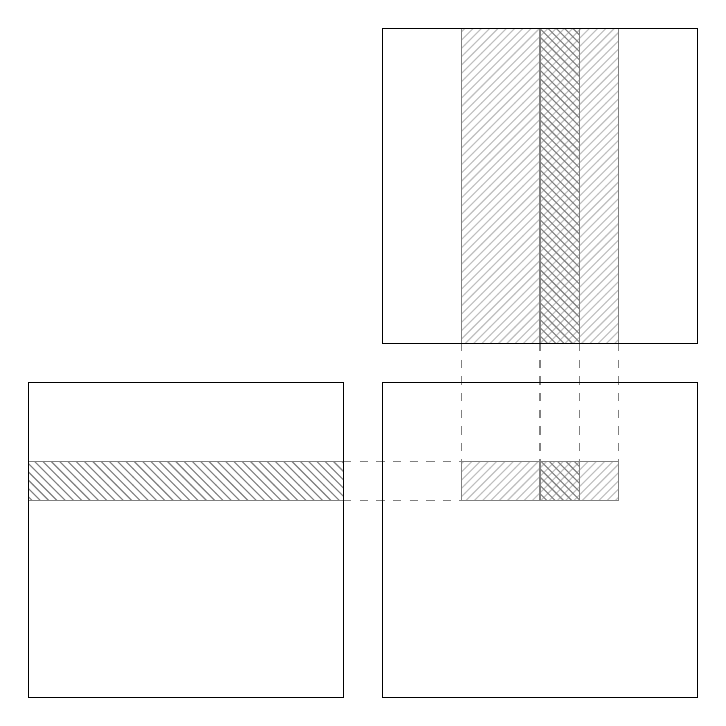
\begin{tikzpicture}[scale=0.5]
        % Cached areas
        \draw[gray, pattern=north east lines, pattern color=gray!50] (2.5, 0.5) rectangle +(4, 8);
        \draw[gray, pattern=north east lines, pattern color=gray!50] (2.5,-3.5) rectangle +(4, 1);

        % Work areas
        \draw[gray, pattern=north west lines, pattern color=gray] ( 4.5, 0.5) rectangle +( 1, 8);
        \draw[gray, pattern=north west lines, pattern color=gray] ( 4.5,-3.5) rectangle +( 1, 1);
        \draw[gray, pattern=north west lines, pattern color=gray] (-0.5,-3.5) rectangle +(-8, 1);

        \draw[gray, dashed] (-0.5, -2.5) -- +(3, 0);
        \draw[gray, dashed] (-0.5, -3.5) -- +(3, 0);
        
        \draw[gray, dashed] (2.5, 0.5) -- +(0, -3);
        \draw[gray, dashed] (4.5, 0.5) -- +(0, -3);
        \draw[gray, dashed] (5.5, 0.5) -- +(0, -3);
        \draw[gray, dashed] (6.5, 0.5) -- +(0, -3);

        \draw ( 0.5,  0.5) rectangle +( 8,  8);
        \draw ( 0.5, -0.5) rectangle +( 8, -8);
        \draw (-0.5, -0.5) rectangle +(-8, -8);
    \end{tikzpicture}
    \label{fig:mm_cache_footprint}
    \caption{
        Calculating a single element in a matrix multiplication can exploit the cheaper memory accesses on the same cachelines. 
    }
\end{figure}

A matrix multiplication of $A \cdot B = C$ with $C$ being of size $I_w \times I_h$, and $A$ and $B$ being size $I_w \times D$ and $D \times I_h$ respectively, we compute the lower bound on the required cache by seperating the horizontal and vertical reads.

\begin{figure}
    \centering
    \begin{tikzpicture}[spy using outlines={rectangle, magnification=4,connect spies}]
        \node (image) at (0,0) {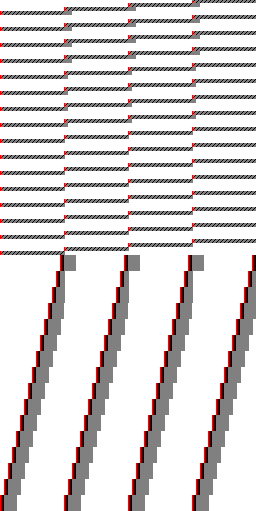
\includegraphics[width=0.25\textwidth]{st_diagrams/matrix_column_4.png}};
        \draw [->] (image.south west) -- ++(2,0) node[right]{\footnotesize\textit{Time}};
        \draw [->] (image.south west) -- ++(0,8.5) node[rotate=90, above left]{\footnotesize\textit{Memory Addresses}};

        \coordinate (p) at (0, 1);
        \coordinate (v) at (3.3, 2);
        \spy[width=2.4cm,height=4cm] on (p) in node [fill=white] at (v);
    \end{tikzpicture}
    \caption{
        The spatial temporal diagram of a matrix multiplication with a column of size 4 ordering.
        See section \ref{sec:st_analysis}.
    }
    \label{fig:st_matrix_column}
\end{figure}


\[
    M_{l} = \ceil{\frac{d}{L}} + d\ceil{\frac{c}{L}}
\]

Similarly to stencil operations, approximate $M_{size}$ using the asymptote

\[
    M_{size} = u h c 
\]

Then solving for $c$

\[
    c = \frac{M_{size}}{u h}
\]


\chapter{Results}
\TODO{Benchmark results, Nvidia profiler statistics}
\section{CUDA Benchmarks}

We run the remapping on two simple CUDA programs: a $9 \times 9$ stencil operation on a $4096 \times 4096$ input, and a matrix multiplication on two $4096 \times 4096$ arrays of 32-bit floating point numbers.
Contrary to our expectations, the kernel execution time seems to be not correlated to our estimated column width at all, instead prefering lower multiple of 32 widths regardless of block size (figure \ref{fig:cuda_kernel_times}).
The factor of 32 seems to be independent of input size and upholds during non power of 2 inputs (figure \ref{fig:cuda_kernel_time_stencil_no_pow2}).
Changing the data type to half precision (16-bit) floating points had effect on the overal improvements.
Using 64-bit double precision floating points made the kernel compute bound instead of memory bound and therefore no tangible difference between the naive implementation and any column remapping is observed.
This exeggerates our earlier assumption (section \ref{sec:implementation_theory}) that the 32 thread wide warps might play a role.

\begin{figure}[b]
    \centering
    \makebox[\textwidth][c] {
        \subfloat[The execution time in milliseconds of a $9 \times 9$ stenciling kernel on a $4096 \times 4096$ input array with various column sizes and block sizes (prefixed with \textit{b}).]{
            \centering
            \pgfplotstabletypeset[col sep=comma,
                /color cells/max=1.3,
                /color cells/min=4.2,
                /color cells/textcolor=black,
                columns/b32/.style={color cells},
                columns/b64/.style={color cells},
                columns/b128/.style={color cells},
                columns/b256/.style={color cells},
                columns/b512/.style={color cells},
                columns/b1024/.style={color cells},
                columns/bench/.style={string type},
                /pgfplots/colormap name=viridis-light]{kernel_time_stencil.csv}
        }
        \label{fig:cuda_kernel_time_stencil}
        \qquad
        \subfloat[The execution time in milliseconds of matrix multiplications on two $4096 \times 4096$ input arrays with various column sizes and block sizes (prefixed with \textit{b}).]{
            \centering
            \pgfplotstabletypeset[col sep=comma,
                /color cells/max=1.7,
                /color cells/min=4.2,
                /color cells/textcolor=black,
                columns/b32/.style={color cells},
                columns/b64/.style={color cells},
                columns/b128/.style={color cells},
                columns/b256/.style={color cells},
                columns/b512/.style={color cells},
                columns/b1024/.style={color cells},
                columns/bench/.style={string type},
                /pgfplots/colormap name=viridis-light]{kernel_time_matrix.csv}
        }
    }
    \label{fig:cuda_kernel_time_matrix}
    \caption{
        asda
    }
    \label{fig:cuda_kernel_times}
\end{figure}

\begin{figure}
    \centering
    \pgfplotstabletypeset[col sep=comma,
        /color cells/max=1.25,
        /color cells/min=4.2,
        /color cells/textcolor=black,
        columns/b32/.style={color cells},
        columns/b64/.style={color cells},
        columns/b128/.style={color cells},
        columns/b256/.style={color cells},
        columns/b512/.style={color cells},
        columns/b1024/.style={color cells},
        columns/bench/.style={string type},
        /pgfplots/colormap name=viridis-light]{kernel_time_stencil_4037.csv}
    \caption{The execution time in milliseconds of a $9 \times 9$ stenciling kernel on a $4037 \times 4037$ input array with various column sizes and block sizes (prefixed with \textit{b}). Even on non power of two's, column widths of multiples of 32 produce more optimal results.}
    \label{fig:cuda_kernel_time_stencil_no_pow2}
\end{figure}

\begin{figure}
    \centering
    \begin{tikzpicture}
        \begin{axis}[
            xlabel = Input Size,
            ylabel = Execution time compared to naive,
            xmode = log,
            ymajorgrids,
            %log ticks with fixed point,
            log basis x={2},
            xmin=128,
            xmax=8192,
            xtick={128,256,512,1024,2048,4096,8192},
            colormap name=viridis,
            cycle list={[colors of colormap={0, 150,..., 1000}]},
            every axis plot/.append style={thick},
            legend pos=north west,
            height=10cm,
        ]
            \addplot[mark=none, black, samples=2, domain=128:8192] {1};
            \addlegendentry{Naive}
            \addlegendimage{empty legend}
            \addlegendentry[yshift=10pt]{\textbf{Column}}
            \pgfplotsinvokeforeach{32, 64, 128, 256, 512, 1024, 2048} {
                \addplot table[
                    x = size,
                    y expr  = \thisrow{c#1}/\thisrow{c0},
                    col sep = comma,
                ]{kernel_time_vs_input_stencil.csv};
                \addlegendentry{#1}
            }
        \end{axis}
    \end{tikzpicture}
    \caption{
        The relative kernel execution time of various column widths compared to the naive implementation for a $9 \times 9$ stencil operation on an $N \times N$ matrix. Lower is better.
    }
\end{figure}

\begin{figure}
    \centering
    \begin{tikzpicture}
        \begin{axis}[
            xlabel = Input Size,
            ylabel = Execution time compared to naive,
            xmode = log,
            ymajorgrids,
            %log ticks with fixed point,
            log basis x={2},
            xmin=128,
            xmax=2048,
            xtick={128,256,512,1024,2048},
            colormap name=viridis,
            cycle list={[colors of colormap={0, 150,..., 1000}]},
            every axis plot/.append style={thick},
            legend pos=south west,
            height=10cm,
        ]
            \addplot[mark=none, black, samples=2, domain=128:8192] {1};
            \addlegendentry{Naive}
            \addlegendimage{empty legend}
            \addlegendentry[yshift=10pt]{\textbf{Column}}
            \pgfplotsinvokeforeach{32, 64, 128, 256, 512, 1024, 2048} {
                \addplot table[
                    x = size,
                    y expr  = \thisrow{c#1}/\thisrow{c0},
                    col sep = comma,
                ]{kernel_time_vs_input_matrix.csv};
                \addlegendentry{#1}
            }
        \end{axis}
    \end{tikzpicture}
    \caption{
        The relative kernel execution time of various column widths compared to the naive implementation for the matrix multiplication of two $N \times N$ matrices. Lower is better.
    }
\end{figure}

\section{Execution Times}
\section{Cache Hitrate}
\section{Hardware Utilization}

\chapter{Conclusion}

\bibliographystyle{unsrtnat}
\bibliography{bibliography}
\end{document}
